%% The first command in your LaTeX source must be the \documentclass command.
%%
%% Options:
%% twocolumn : Two column layout.
%% hf: enable header and footer.
\documentclass[
% twocolumn,
% hf,
]{ceurart}

%%
%% One can fix some overfulls
\sloppy

%%
%% Minted listings support 
%% Need pygment <http://pygments.org/> <http://pypi.python.org/pypi/Pygments>
\usepackage{subcaption}
\usepackage{pdfpages}
\usepackage[colorinlistoftodos]{todonotes}
%% auto break lines
\usepackage{amsmath,amssymb,amsfonts}
\usepackage{algorithmic}
\usepackage{graphicx}
\usepackage{textcomp}
\usepackage{xcolor}
\usepackage{svg}
\usepackage{enumitem}
\usepackage{hyperref}
\usepackage{listings}

\lstdefinestyle{sparqlstyle}{
    basicstyle=\ttfamily\footnotesize,
    breakatwhitespace=false,         
    breaklines=true,                 
    keepspaces=true,                 
    showspaces=false,      
    captionpos=b,
    showstringspaces=false,
    showtabs=false,                  
    tabsize=2
}
\lstset{style=sparqlstyle}
\def\BibTeX{{\rm B\kern-.05em{\sc i\kern-.025em b}\kern-.08em
    T\kern-.1667em\lower.7ex\hbox{E}\kern-.125emX}}

%%
%% end of the preamble, start of the body of the document source.
\begin{document}

%%
%% Rights management information.
%% CC-BY is default license.
\copyrightyear{2024}
\copyrightclause{Copyright for this paper by its authors.
  Use permitted under Creative Commons License Attribution 4.0
  International (CC BY 4.0).}

%%
%% This command is for the conference information
\conference{D2R2’24 Third International Workshop on Linked Data-driven Resilience Research co-located with ESWC 2023, May 27th, 2024, Hersonissos, Greece}

%%
%% The "title" command
\title{COCONUT-KG: Publishing a Large Collection of Open Natural Products over Linked Data}

%\tnotemark[1]

%%
%% The "author" command and its associated commands are used to define
%% the authors and their affiliations.
\author[1]{István J. Mócsy}[%
email=istvan.mocsy@stud.htwk-leipzig.de,
]
\cormark[1]
% \fnmark[1]
\address[1]{AKSW, Leipzig University of Applied Sciences (HTWK),
  Gustav-Freytag-Straße 42a, Leipzig, 04277, Germany}

\author[1]{Paulo Viviurka do Carmo}[%
email=paulo.carmo@htwk-leipzig.de,
]

\author[1]{Edgard Marx}[%
email=edgard.marx@htwk-leipzig.de,
]

\author[1]{Stefan Schmidt-Dichte}[%
email=stefan.schmidt-dichte@stud.htwk-leipzig.de,
]

% \fnmark[1]



%% Footnotes
\cortext[1]{Corresponding author.}
% \fntext[1]{These authors contributed equally.}

%%
%% The abstract is a short summary of the work to be presented in the
%% article.
\begin{abstract}
We need to follow this paper as example \url{https://arxiv.org/pdf/2009.06337.pdf} for D2R2 \url{https://ceur-ws.org/Vol-3401/paper1.pdf}
\end{abstract}

%%
%% Keywords. The author(s) should pick words that accurately describe
%% the work being presented. Separate the keywords with commas.
\begin{keywords}
  Knowledge Engineering \sep
  Linked Data \sep
  Natural Products \sep
  Knowledge Graphs \sep
  CEUR-WS
\end{keywords}

%%
%% This command processes the author and affiliation and title
%% information and builds the first part of the formatted document.
\maketitle

\section{Introduction}

Knowledge Graphs (KGs) allow data to be published in a structured manner for many different applications~\cite{hogan2021knowledge}.
KGs structure are based on an ontology that maps the data properties into a triple system in the form of $subject \rightarrow predicate \rightarrow object$, which is described by the Resource Description Framework (RDF).
KGs allow the data to be queried by a standard language like SPARQL whenever they are made available by endpoints, data managements frameworks (e.g. KBox~\cite{marx2017kbox}), and/or URI-dataset indices (e.g. WIMUQ~\cite{valdestilhas2019more}).
SPARQL allows the users to query KGs by available enpoints, while combining all the necessary KGs and ontologies to obtain all the data you need, with filters and restrictions.
These capabilities allow the existence of specific and broader KGs like DBpedia~\cite{lehmann2015dbpedia}, Freebase~\cite{bollacker2008freebase} and YAGO2~\cite{hoffart2013yago2}.

In this paper we are interested on developing and maintaining a natural products KG.
We refer to natural products as chemical compounds generated by living organisms, which contribute to as much as 67\% of the drugs approved worldwide~\cite{newman2016natural}.
Natural products databases contain data like descriptions, molecules, usage, characteristics and even from which species and location they are extracted from.
More specifically, in this paper we present the process of devoloping the KG version of the COlleCtion of Open Natural ProdUcTs (COCONUT)~\cite{sorokina2021coconut} database.
There are many others natural products databases like NPAtlas~\cite{van2019natural,van2022natural}, PubChem~\cite{kim2023pubchem}, and NuBBE$_{DB}$~\cite{valli2013development,pilon2017nubbedb}.
However, the COCONUT database is an open source project for natural products, search and analysis by gathering over 50 open natural product resources and is available for free without any restriction.
Therefore, we chose it for developing a KG version.

We developed a KG for the COCONUT database called COCONUT[KG]\footnote{Accessible at: \url{http://coconut-kg.aksw.org}}, by following three steps: (i) extraction and exploration of the COCONUT data for better understanding; (ii) depevelopment of the ontology and tranformation for a KG; and (iii) publication of an endpoint and documentation surrounding the KG.
Table \ref{tab:resources} presents the resources described by this paper.

\textcolor{red}{paulo: I think we can save some space here by just re-directing people and no resource description}

\begin{table}[h]
    \centering
    \caption{Resources described in this paper.}
    \label{tab:resources}
    \resizebox{.6\linewidth}{!}{
        \begin{tabular}{r|l|l}
        \hline
        Resource & URL & License \\
        \hline\hline
             Ontology & \url{http://coconut-kg.aksw.org/ontology} & \href{https://creativecommons.org/licenses/by-sa/4.0/}{CC BY-SA 4.0} \\ \hline
             Dataset  &  \url{http://coconut-kg.aksw.org/dataset} & \href{https://creativecommons.org/licenses/by-sa/4.0/}{CC BY-SA 4.0} \\ \hline
             Endpoint  &  \url{http://coconut-kg.aksw.org/query} & \href{https://creativecommons.org/licenses/by-sa/4.0/}{CC BY-SA 4.0} \\
             \hline
        \end{tabular}
    }
\end{table}

\section{Dataset}
\begin{itemize}
    \item Original dataset comes as MongoDB dump
    \item Export of hole Dataset to JSON files
    \item We used the \texttt{sourceNaturalProduct.json} in the following process
    \item Why?
    \begin{itemize}
        \item contains the information of other files like \texttt{uniqueNaturalProduct.json}
    \end{itemize}
    \item Exploration of the JSON file to find canidates for possible classes and properties
\end{itemize}

\textcolor{red}{paulo: gonna make an image of this workflow so we can save space on describing explanations. also think we'll need to not use the table of stats}

\begin{table}[h]
    \centering
    \caption{Coconut Knowledge Graph domain statistics.}
    \label{tab:subsets}
    \resizebox{.98\linewidth}{!}{
        \begin{tabular}{r|r|r|r|r}
        \hline
        Domain &  \#Classes & \#Object Properties & \#Data Properties & \#Instances\\
        \hline\hline
             Molecule & Taxonomy & & 2 & 1536262 \\
            & Geolocation & & 1 & 1536262 \\
            & ConstitutionalDescriptors & & 7 & 1536262 \\
            & UniqueIdentifiers & & 14 & 1536262 \\
            & MolecularFragments & & 4 & 1536262 \\
            & ElectronicDescriptors & & 4 & 1536262 \\
            & GeometricalDescriptors& & 1 & 1536262 \\
            & Descriptors & 5 & &  1536262 \\
            & Compound & 10 & 5 & 1536262 \\
            & Fingerprint &  & 5 & 1536261 \\
            & MolecularFeatures &  & 3 & 1536261 \\
            & MolecularProperties &  & 11 & 1536260 \\
            & MolecularDescriptors &  & 4 & 1536260 \\
            & TopologicalDescriptors &  & 13 & 1536260 \\ \hline
             Publishment  &  \#DataOriginSource & & 6 & 1536260 \\ 
             & \#Citation & & 1 & 1536262 \\ \hline\hline
             Total & 16 & 15 & 80 & 1536262 \\ \hline
        \end{tabular}
    }
\end{table}

\section{The Data Model}

In the version 1.0.0 of our data model, all classes are build around the class coco:Compound and are attempting to categorize the various properties of a compound. Following, we will give an insight of the classes. \\

%\textcolor{red}{paulo: I'm having a problem reading the text on the image, specially the properties.}

%\textcolor{red}{Istvan: Should be better now}
\textcolor{red}{Stefan: Some thoughts about the schema: "is Electronic" is the only predicate written with a capital letter? Is it on purpose? I'm not so sure right now that I don't like "has ... descriptor" better. Somehow I find that e.g. "is topological" reads strange (From the perspective of natural language). It is then e.g. Descriptors $\longrightarrow$ is molecular $\longrightarrow$ Molecular-descriptors. Other opinions? I am really not sure and would like to know your opinion.}

\textcolor{red}{Istvan: The capital E has been fixed, was just an overseen typo. the "is ..." on the other hand seems correct to me}
\begin{figure*}[ht]
    \centering
    \includesvg[inkscapelatex=false, width=\textwidth]{schema1_0_0.svg}
    \caption{The current class structure of the coconut-kg schema}
    \label{fig:classes_coco}
\end{figure*}

\begin{enumerate}[label=\emph{\alph*})]

\item \textit{Descriptors:} Collects all of the descriptors of a compound. There are constitutional, electronic, molecular, geometrical and topological descriptors.

\item \textit{Molecular properties:} All properties, which describe the basics of a given compound.

\item \textit{Molecular features:} Information regarding sugar containment of a compound.

\item \textit{Unique identifiers:} Identifiers which are used to exactly identify a compound, like Simplified Molecular Input Line Entry Specifications(SMILES) and International Chemical Identifier(inchi) keys.

\item \textit{Fingerprint:} Fingerprint sequences and bitstrings of the compound from various databases.

\item \textit{Geolocation:} Location information by continent.

\item \textit{Data origin source:} The Coconut database is a collection of multiple natural producs databases. The information about when and where coconut has extracted the data is held here.

\item \textit{Citation:} Any literature a compound has been mentioned in.

\item \textit{Taxonomy:} Taxonomy information of the compound.

\end{enumerate}

Followed by an overview of the data properties and their counts in the current v1.0.0 dataset:


\textcolor{red}{Stefan: we should check if e.g. taxonomyReferenceObjects occurs less than once, otherwise we could remove it from the data and document it. And maybe remove the "is..." things from the graphic}

\textcolor{red}{Istvan: taxonomyReferenceObjects seems to occur less than once/has empty values in it. Added to improvements page}

\begin{figure*}
    \centering
    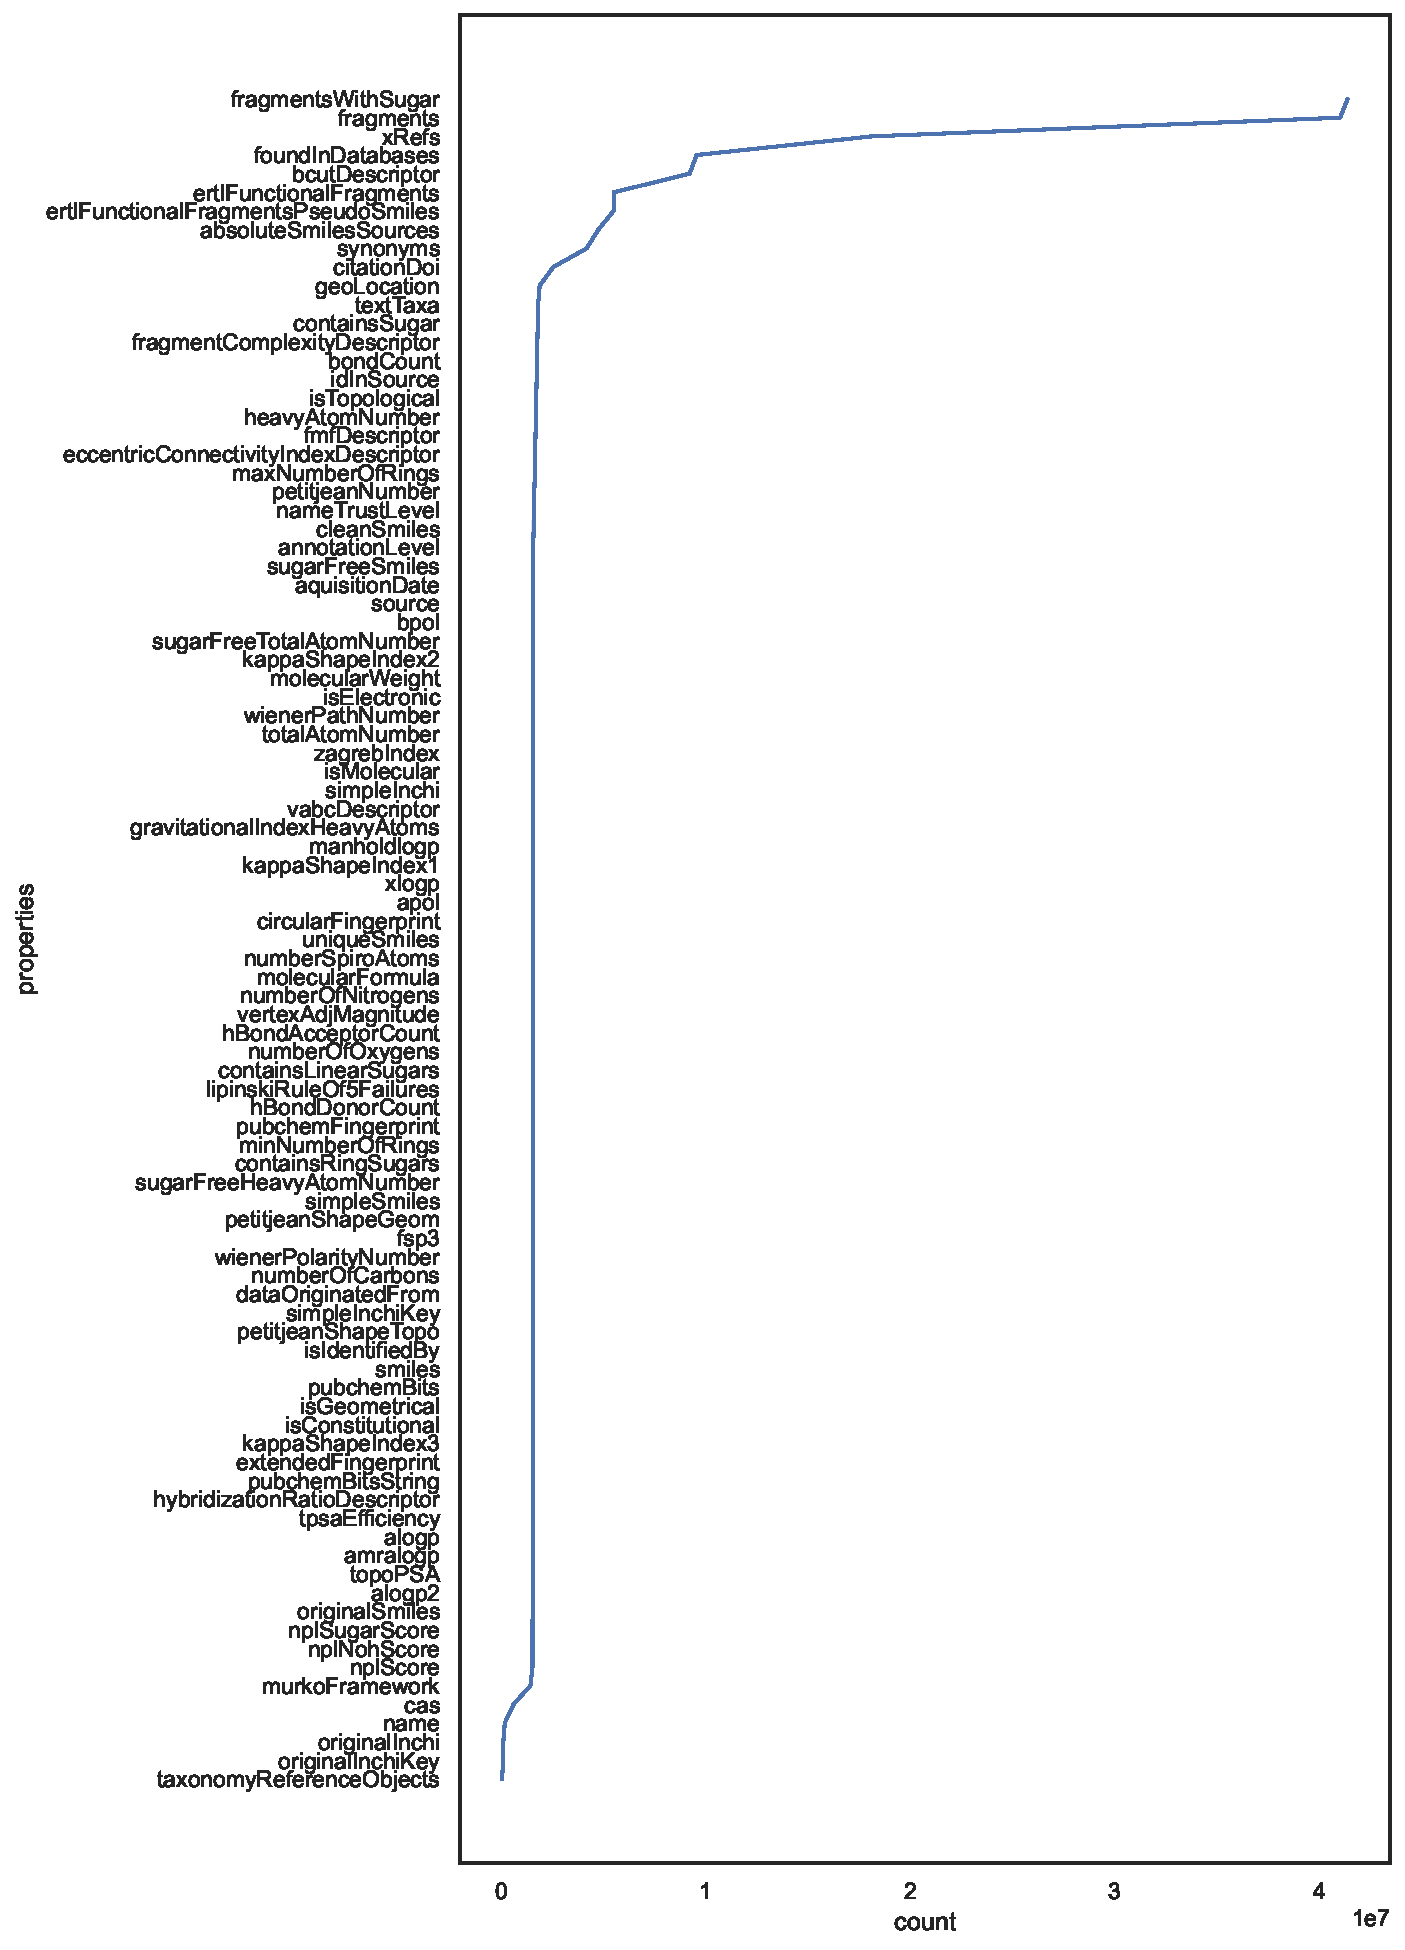
\includegraphics[width=\textwidth]{properties_plot_v1.0.0.pdf}
    \caption{All properties counted up to 1e7}
    \label{fig:propertiescount}
\end{figure*}



\section{Exploring}
To allow our KG to be accessed and queried, we published an endpoint using OpenLink Virtuoso Open-Source Edition~\cite{erling2012virtuoso}. We also provided a YASGUI~\cite{rietveld2017yasgui} SPARQL query editor~\footnote{Accessible at: \url{http://coconut-kg.aksw.org/query}} for a more user-friendly experience.
To explore the data, a SPARQL query has to be sent to the endpoint. A regular query already specifies the parts of the data that a user wants to accesss.
In the example query below~\ref{lst:query1} we ask to list the molecular formula, the name, the weight and the smile of the first 1000 compounds of our dataset.

\begin{lstlisting}[language=sparql, label=lst:query1, caption=Example SPARQL query]
PREFIX coco:  <http://coconut-kg.aksw.org/ontology#>
PREFIX rdf:  <http://www.w3.org/1999/02/22-rdf-syntax-ns#>
PREFIX rdfs: <http://www.w3.org/2000/01/rdf-schema#>
PREFIX owl:  <http://www.w3.org/2002/07/owl#>
PREFIX xsd:  <http://www.w3.org/2001/XMLSchema#>

SELECT DISTINCT ?formula ?name ?weight ?smile WHERE {
?compound a coco:Compound .
?compound coco:molecularFormula ?formula .
?compound coco:name ?name .

?compound coco:hasDescriptors ?descriptor .
?descriptor coco:isMolecular ?mdescriptor .
?mdescriptor coco:molecularWeight ?weight .

?compound coco:isIdentifiedBy ?unique .
?unique coco:smiles ?smile .}

LIMIT 1000
\end{lstlisting}

More query examples for our dataset specifically can be found in our documentation~\footnote{Accessible at: \url{http://coconut-kg.aksw.org/about/query}}.

\begin{table}[h]
    \centering
    \caption{Average execution time statistics for Query \ref{lst:query1}.}
    \label{tab:execution time}
    \resizebox{.4\linewidth}{!}{
        \begin{tabular}{l|c}
        \hline
        Limit & Execution time \\
        \hline\hline
        10,000 & 0.6592 $\pm$ 0.1518 \\
        25,000 & 1.4065 $\pm$ 0.1329 \\
        100,000 & 8.4693 $\pm$ 1.1743 \\
        Unlimited (164,121) & 15.615 $\pm$ 3.0062 \\
        \hline
        \end{tabular}
    }
\end{table}


\section*{Acknowledgment}

This work has been partially supported by the German Research Foundation (DFG) and São Paulo State Research Support Foundation (FAPESP) under the project DINOBBIO (DFG Project number 459288952) \url{https://dinobbio.aksw.org}.

%%
%% Define the bibliography file to be used
\bibliography{sample-ceur}


\end{document}

%%
%% End of file
